%!TEX root = ../main.tex

\chapter{Results}\label{cha:results}

In this chapter several fingerprints will be examined in detail.
In Section \ref{sec:tft} a breakdown of the fingerprint for TitForTat is given with an explanation of its appearance.
%TODO
Section \ref{sec:GBM} shows several plots for the strategy GoByMajority, with a varying parameter.
As the parameter changes, a continuous deformation of the plot of the
fingerprint can be observed.
Finally, in Section \ref{sec:lse} we compare the underlying data for all fingerprints of strategies within Axelrod-Python.
This data is used to produce a heat plot of strategies similarity.

It may be useful to recall that a fingerprint for a strategy is produced by playing it against varying stochastic transformations of a probe.
The parameters varied are $x$ and $y$, as seen on fingerprints in this section.
High $x$ values correspond to high cooperation.
Conversely, high $y$ values correspond to high defection.
The colour at point $\hat{x}, \hat{y}$ on the plot indicates the expected value of the strategy when played against the transformation of the probe with parameters $\hat{x}, \hat{y}$.
This expected score has been approximated as outlined in Chapter \ref{cha:implementation}.


\section{Interpretation of TFT}\label{sec:tft}
TitForTat (see Section \ref{ssec:stra_titfortat} for an explanation of its behaviour) it is one of the most well known strategies for Prisoner's Dilemma.
Also, it produces a clean and easy to understand fingerprint, shown in Figure \ref{fig:TFT}, making it an ideal place to start.
% TODO You need to say who the probe was?

\begin{figure}[hbtp!]
\centering
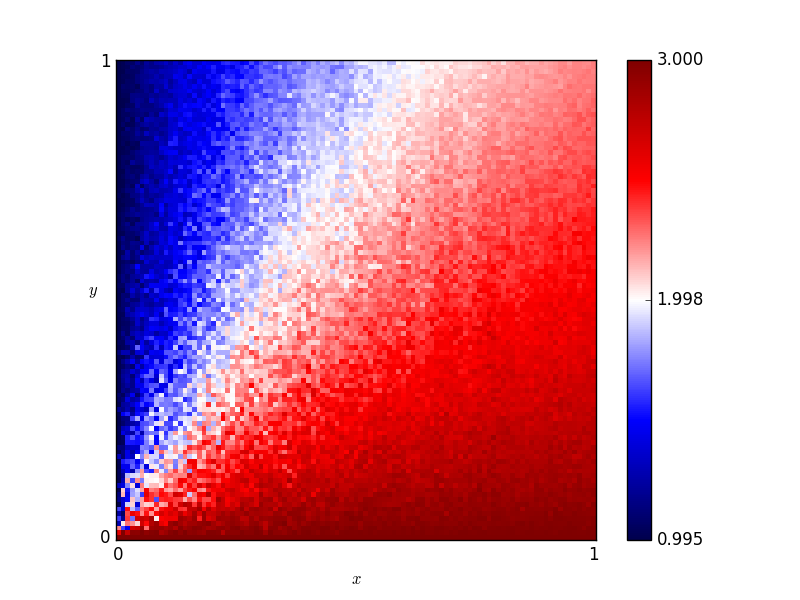
\includegraphics[width = 0.6\textwidth]{../img/Numerical/Tit_For_Tat.png}
\caption{Fingerprint for TitForTat, with colour bar to add context}
% TODO The colour bar is default in 2.6 right?
% Go back and check that any fingerprints have the colour bar and that any
% discussion makes it clear.
\label{fig:TFT}
\end{figure}

The plot slowly transitions from a strip of blue in the top left, rotating around to a large block of red in the bottom right.
The blue area corresponds to low scores and it can be seen that this occurs for small values of $x$.
However, as $x$ increases higher scores (shown in red) quickly take over.
This is exactly as expected, TitForTat plays well in highly cooperative environments.
An immediate question is; why does the white stripe not follow the diagonal?
The main diagonal is where $x=y$ and due to the random nature of the cooperation and defections, the expected average score for TitForTat would be !!!! about half the maximum.
% TODO What is !!!!
Due to the global minimum and maximum that TitForTat achieves, a score of !!!! is not midway, and so the white line showing the middle score is off centre.
% TODO !!!!
TitForTat is able to produce better than half scores in this scenario by encouraging the underlying probe strategy to cooperate.

\section{Varying the parameter for Random}
It is possible to observe how changing a parameter for a strategy will affect its behaviour by comparing the fingerprints for each parameter.
As described in Section \ref{ssec:strat_random}, Random accepts a parameter that determines the probability of cooperation.
We can vary this parameter and create a new fingerprint each time.

\begin{figure}[htbp!]
\centering
\subfloat[Defector]{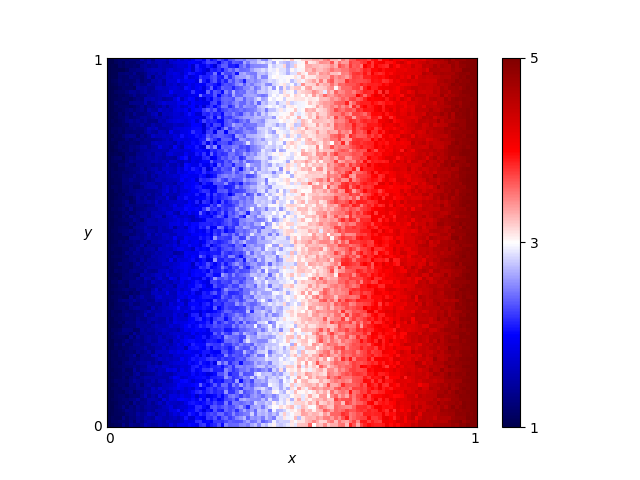
\includegraphics[width = 0.3\textwidth]{../img/Numerical/Defector.png}}\\[-2ex]

\subfloat[Random(0.1) - will cooperate\protect\\10\% of the time]{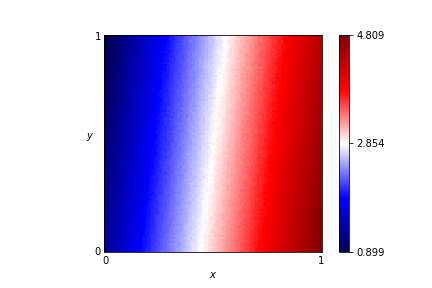
\includegraphics[width = 0.3\textwidth]{../img/Numerical/Random01.png}}
\subfloat[Random(0.2) - will cooperate\protect\\20\% of the time]{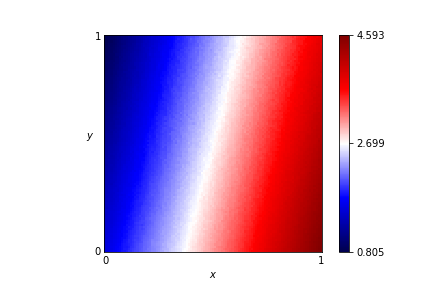
\includegraphics[width = 0.3\textwidth]{../img/Numerical/Random02.png}}
\subfloat[Random(0.3) - will cooperate\protect\\30\% of the time]{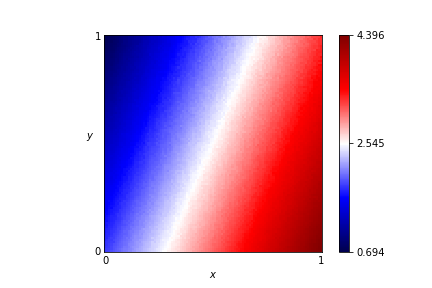
\includegraphics[width = 0.3\textwidth]{../img/Numerical/Random03.png}}\\[-2ex]

\subfloat[Random(0.4) - will cooperate\protect\\40\% of the time]{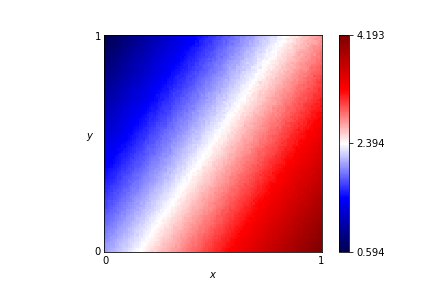
\includegraphics[width = 0.3\textwidth]{../img/Numerical/Random04.png}}
\subfloat[Random(0.5) - will cooperate\protect\\50\% of the time]{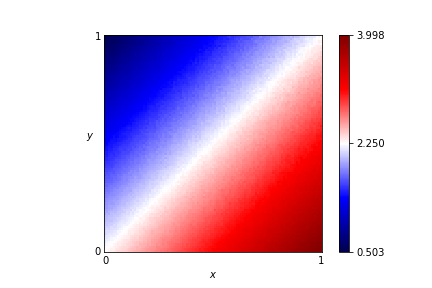
\includegraphics[width = 0.3\textwidth]{../img/Numerical/Random05.png}}
\subfloat[Random(0.6) - will cooperate\protect\\60\% of the time]{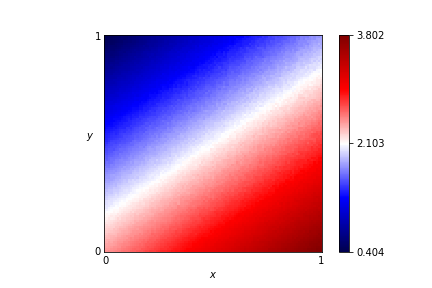
\includegraphics[width = 0.3\textwidth]{../img/Numerical/Random06.png}}\\[-2ex]

\subfloat[Random(0.7) - will cooperate\protect\\70\% of the time]{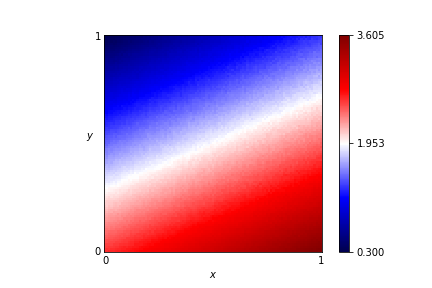
\includegraphics[width = 0.3\textwidth]{../img/Numerical/Random07.png}}
\subfloat[Random(0.8) - will cooperate\protect\\80\% of the time]{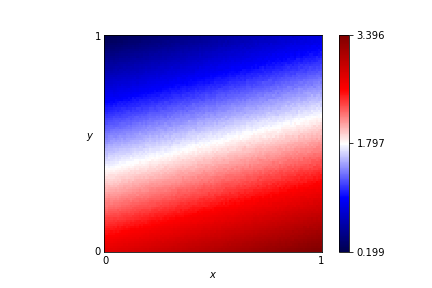
\includegraphics[width = 0.3\textwidth]{../img/Numerical/Random08.png}}
\subfloat[Random(0.8) - will cooperate\protect\\90\% of the time]{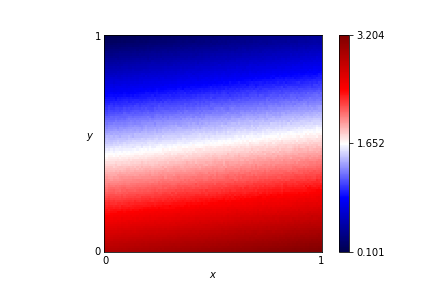
\includegraphics[width = 0.3\textwidth]{../img/Numerical/Random09.png}}\\

\subfloat[Cooperator]{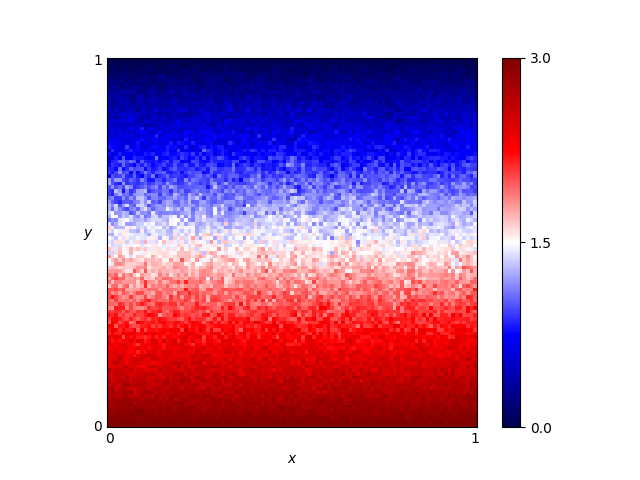
\includegraphics[width = 0.3\textwidth]{../img/Numerical/Cooperator.png}}

\end{figure}



\section{Alternator, Cycler(CD), Cooperator, Defector}

\begin{figure}[htbp!]
    \centering
    \subfloat[Fingerprint for Alternator]{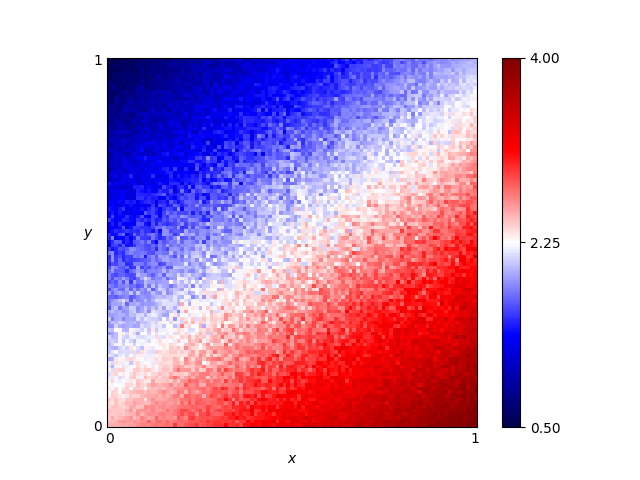
\includegraphics[width = 0.5\textwidth]{../img/Numerical/Alternator.png}}
    \subfloat[Fingerprint for Cycler(CD)]{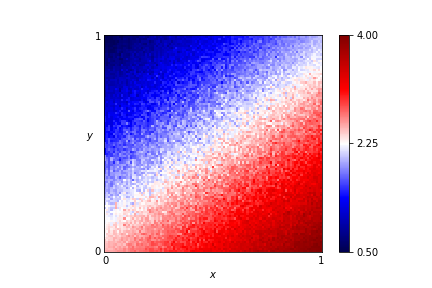
\includegraphics[width = 0.5\textwidth]{../img/Numerical/Cycler_CD.png}}
    \caption{Fingerprints for Alternator and Cylcer(CD) when probed by TitForTat}
    \label{fig:alt_cycler}
\end{figure}

\section{GoByMajority for different parameters}\label{sec:GBM}

\begin{figure}[htbp!]
\subfloat[GoByMajority with memory depth 5]{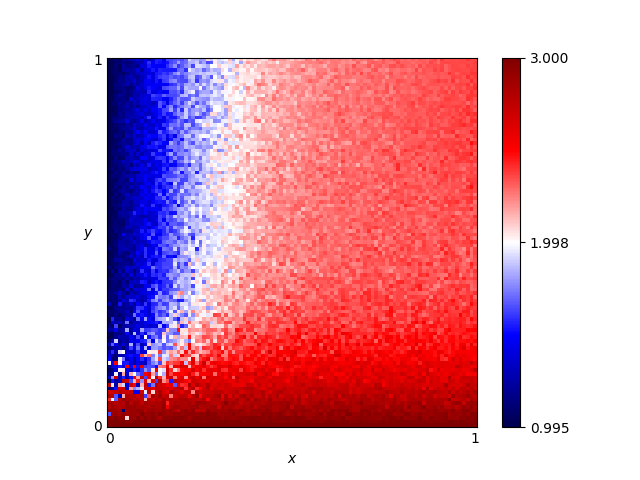
\includegraphics[width = 0.5\textwidth]{../img/Numerical/Go_By_Majority_5.png}}
\subfloat[GoByMajority with memory depth 10]{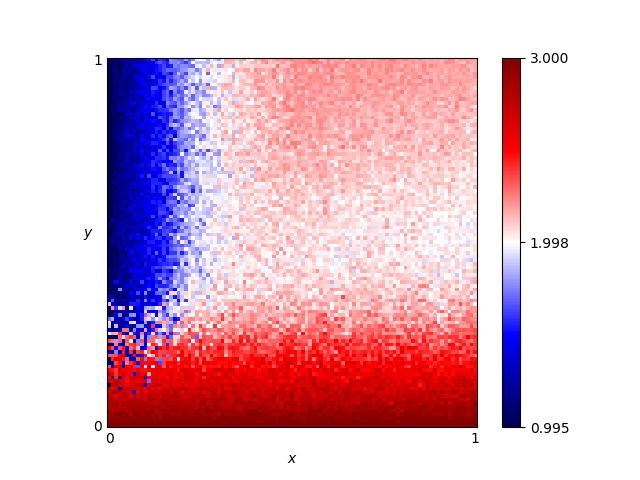
\includegraphics[width = 0.5\textwidth]{../img/Numerical/Go_By_Majority_10.png}}\\
\\
\subfloat[GoByMajority with memory depth 20]{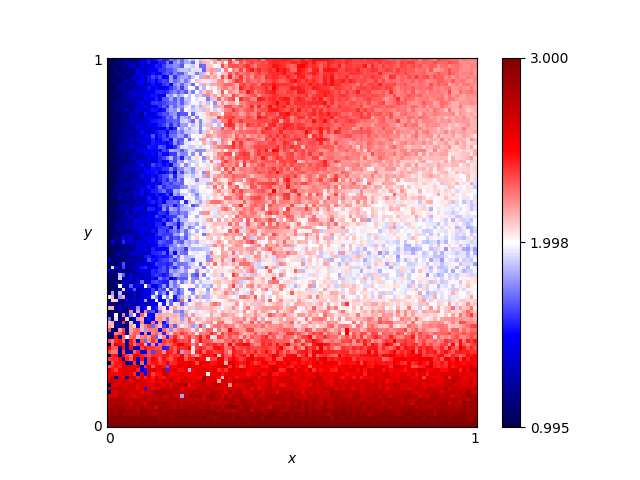
\includegraphics[width = 0.5\textwidth]{../img/Numerical/Go_By_Majority_20.png}}
\subfloat[GoByMajority with memory depth 40]{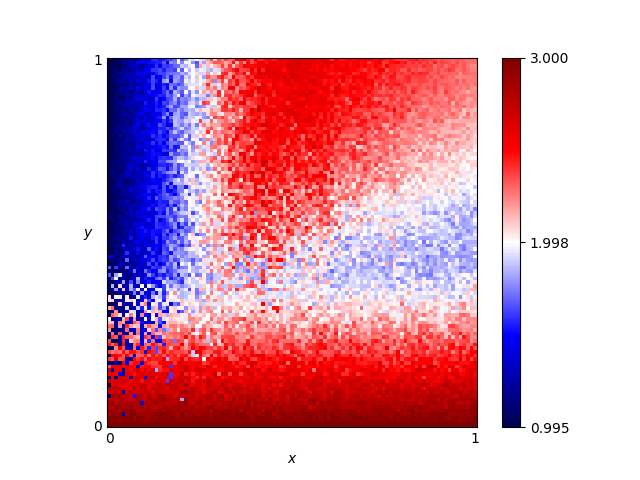
\includegraphics[width = 0.5\textwidth]{../img/Numerical/Go_By_Majority_40.png}}\\
\\
\subfloat[GoByMajority with memory depth 75]{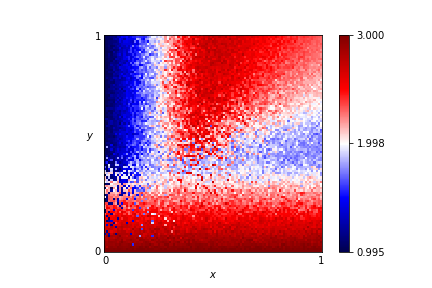
\includegraphics[width = 0.5\textwidth]{../img/Numerical/Go_By_Majority_75.png}}
\subfloat[GoByMajority with memory depth infinite]{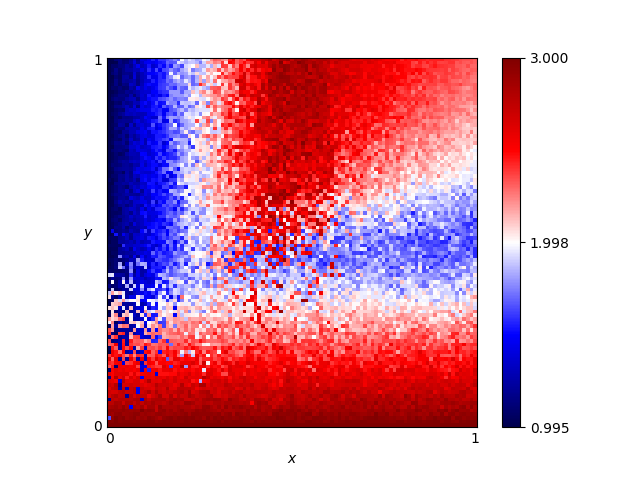
\includegraphics[width = 0.5\textwidth]{../img/Numerical/Go_By_Majority00.png}}
\end{figure}

\section{Random and Cycler(CDDC) with probes TFT and T42T}
The importance of probe selection will now be demonstrated.
Thus far, all fingerprints shown have used TitForTat as a probe, but this is not always enough.
For example, Random and Cycler(CDDC) produce identical fingerprints when probed with TitForTat, as shown in

\begin{figure}[htbp!]
    \centering
    \subfloat[Fingerprint for Random]{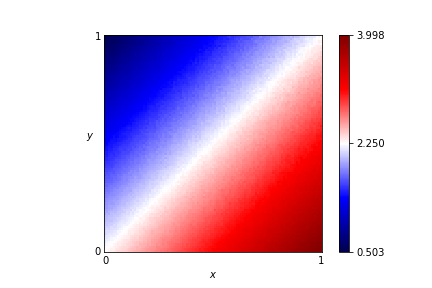
\includegraphics[width = 0.5\textwidth]{../img/Numerical/Random05.png}}
    \subfloat[Fingerprint for Cycler(CDDC)]{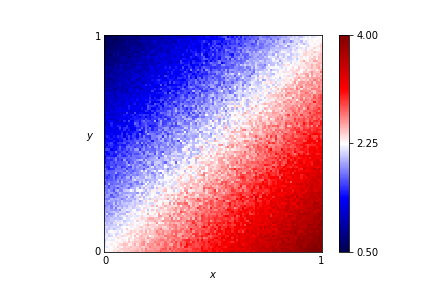
\includegraphics[width = 0.5\textwidth]{../img/Numerical/Cycler(CDDC)_TFT.png}}
    \caption{Fingerprints for Random and Cylcer(CDDC) when probed by TitForTat}
    \label{fig:rand_cycle_tft}
\end{figure}

However, by changing the probe to TitForTwoTats, it becomes obvious that the strategies are different.

\begin{figure}[htbp!]
    \centering
    \subfloat[Fingerprint for Random]{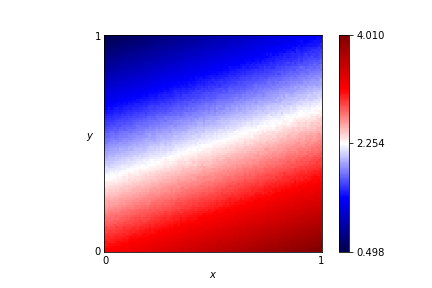
\includegraphics[width = 0.5\textwidth]{../img/Numerical/Random_TF2T.png}}
    \subfloat[Fingerprint for Cycler(CDDC)]{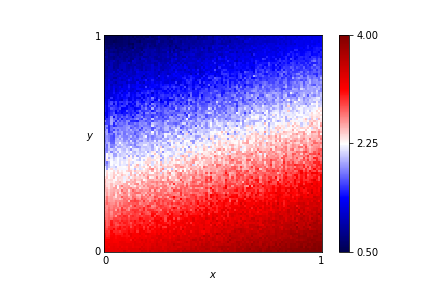
\includegraphics[width = 0.5\textwidth]{../img/Numerical/Cycler(CDDC)_TF2T.png}}
    \caption{Fingerprints for Random and Cylcer(CDDC) when probed by TitForTwoTats}
    \label{fig:rand_cycle_tf2t}
\end{figure}

\begin{figure}[htbp!]
    \centering
    \subfloat[Fingerprint for Random]{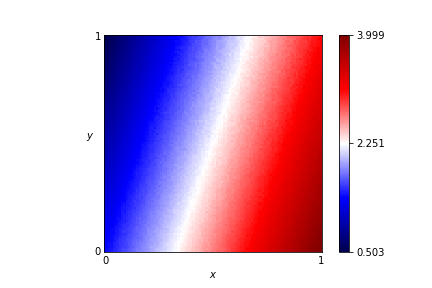
\includegraphics[width = 0.5\textwidth]{../img/Numerical/Random05_2TFT.png}}
    \subfloat[Fingerprint for Cycler(CDDC)]{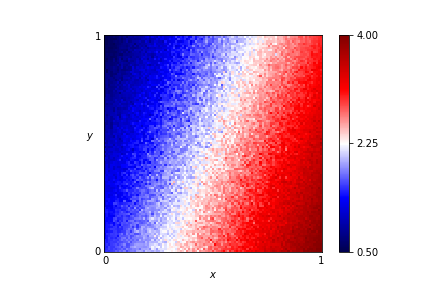
\includegraphics[width = 0.5\textwidth]{../img/Numerical/Cycler_CDDC_2TFT.png}}
    \caption{Fingerprints for Random and Cylcer(CDDC) when probed by TwoTitsForTat}
    \label{fig:rand_cycle_2tft}
\end{figure}

% \begin{figure}[htbp!]
%     \centering
%     \subfloat[Fingerprint for Random]{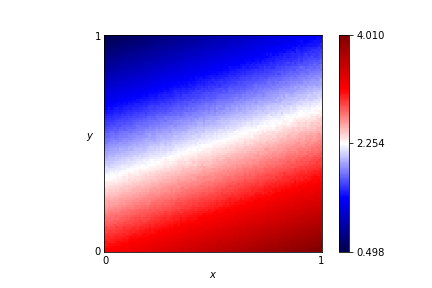
\includegraphics[width = 0.5\textwidth]{../img/Numerical/Random_TF2T.png}}
%     \subfloat[Fingerprint for Cycler(CDDC)]{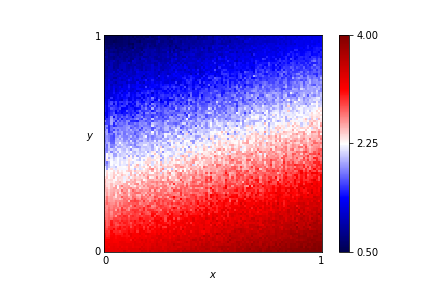
\includegraphics[width = 0.5\textwidth]{../img/Numerical/Cycler(CDDC)_TF2T.png}}
%     \caption{Fingerprints for Random and Cylcer(CDDC) when probed by TitForTwoTats}
%     \label{fig:rrand_cycle_tf2t}
% \end{figure}

\section{LSE plot and table}\label{sec:lse}
